\chapter{МЕТОД STRUCTURE FROM MOTION}

\textbf{Structure from Motion} (дословно \quotes{\textit{структура из движения}}, SFM) - техника построения трёхмерных структур из последовательности двухмерных изображений (фотографий, кадров видео) используемая в области компьютерного зрения. В биологии описывает феномен, позволяющий человеку восстанавливать трёхмерную структуру окружающего мира по двухмерным проекциям на сетчатку глаза.

На рисунке \ref{fig:sfm} представлена схема, демонстрирующая процесс восстанавления 3d модели поверхности.

\begin{figure}[h]
    \centering
    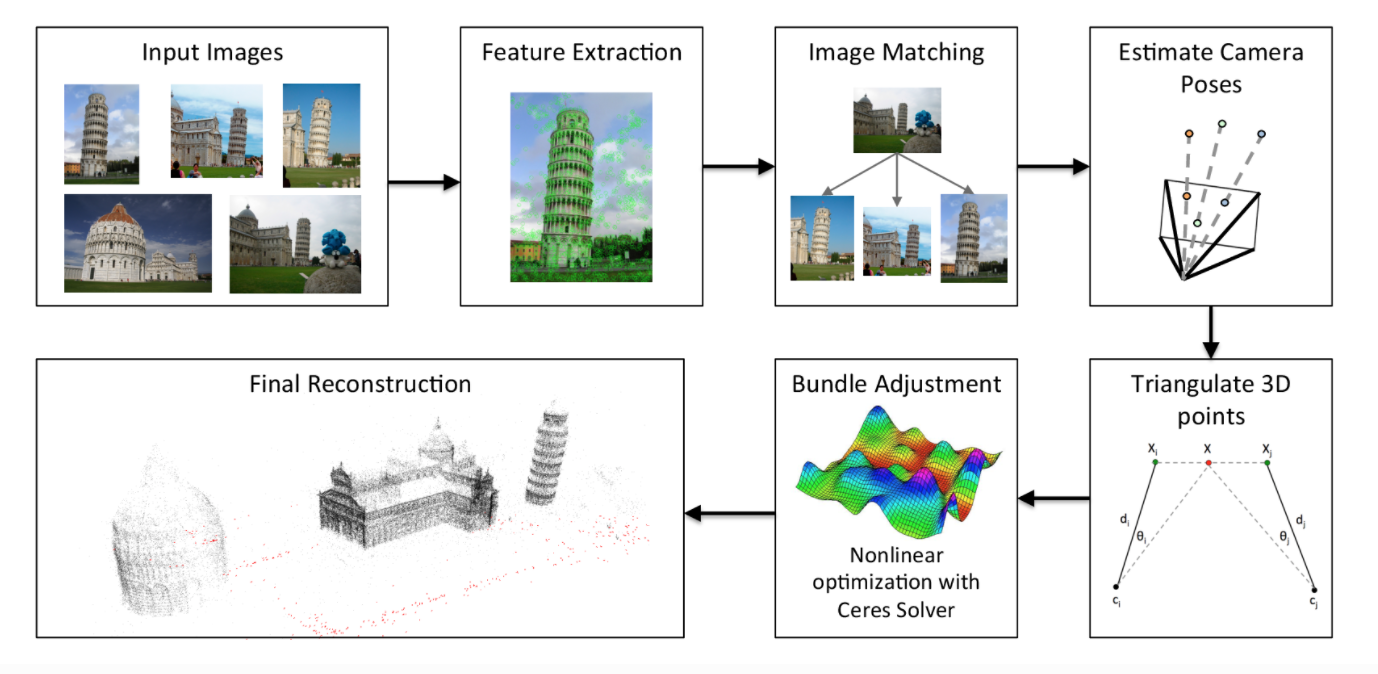
\includegraphics[width=1\textwidth]{sfm.png}
    \caption{\textbf{SFM pipeline}}
    \label{fig:sfm}
\end{figure}

Таким образом можно выделить следующие составляющие процесса реконструкции: 

\begin{enumerate}
    \item Выделение ключевых точек и дескрипторов;
    \item Сравнение дескрипторов и нахождение паросочетаний соответствующих друг другу особых точек;
    \item Нахождение геометрического преобразования, которое переводит ключевые точки одного изображения в соответствующие им точки другого изображения;
    \item Позиционированние камер и расположение их в трехмерном пространстве.
\end{enumerate}

Далее будут подробнее рассмотрены описанные выше этапы и применяемые на них алгоритмы. Для решения первых двух пунктов используются \textit{алгоритмы основанные на особых точках} (\textbf{feature-based algorithms}).
